\subsection{Project Milestones}
\noindent The figure below shows various project milestones with their estimated start and end dates. The duration is given in days. There is also a Gantt chart generated by this data. The paper should be incrementally completed throughout the first semester, progressing towards a subsystem demo before an official full system prototype is made on a breadboard. After that is done, the printed circuit board will be ordered and the entirety of the second semester will be dedicated to integration and final testing and assembly. \\

\begin{figure}[H]
	\centering
	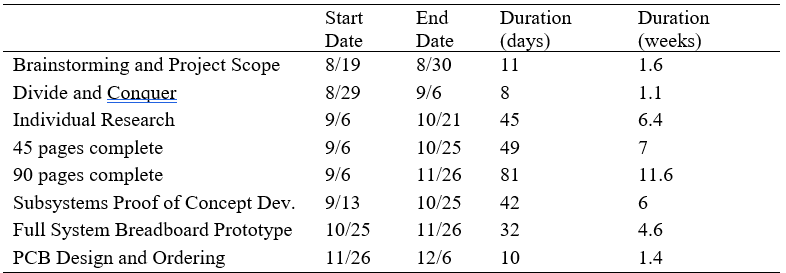
\includegraphics[width=\textwidth]{./Images/SD1mile.png}
	\caption{\label{fig:SD1mile}Senior Design I Milestones}
\end{figure}

\begin{figure}[H]
	\centering
	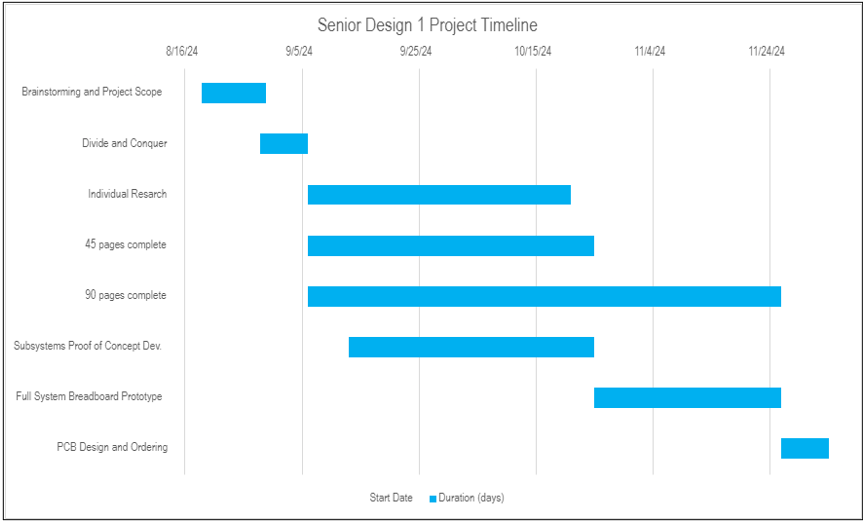
\includegraphics[width=\textwidth]{./Images/SD1gantt.png}
	\caption{\label{fig:SD1gantt}Senior Design I Gantt Chart}
\end{figure}

\begin{figure}[H]
	\centering
	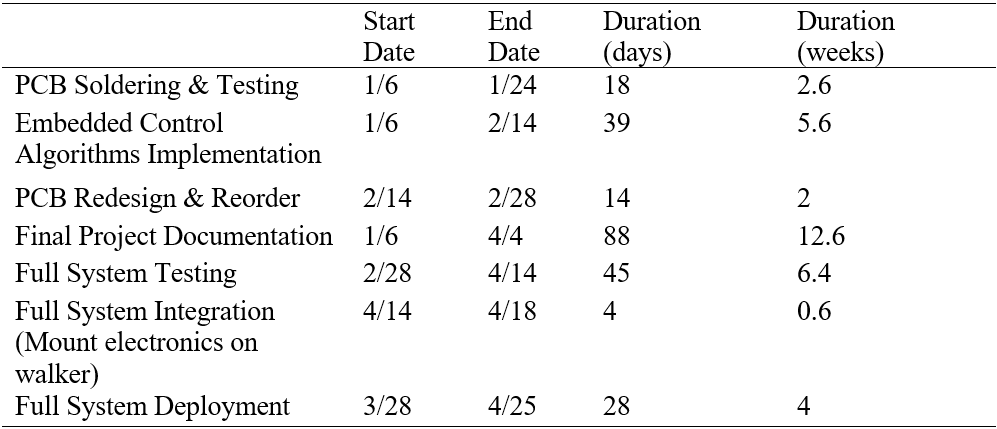
\includegraphics[width=\textwidth]{./Images/SD2mile.png}
	\caption{\label{fig:SD2mile}Senior Design II Milestones}
\end{figure}

\begin{figure}[H]
	\centering
	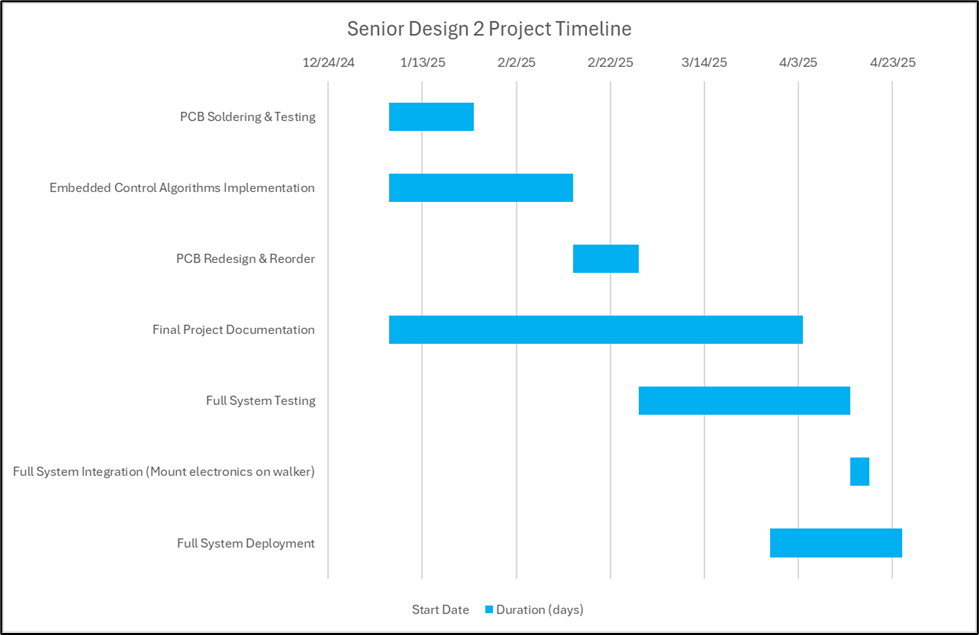
\includegraphics[width=\textwidth]{./Images/SD2gantt.png}
	\caption{\label{fig:SD2gantt}Senior Design II Gantt Chart}
\end{figure}